
A trie, sometimes called a prefix tree, is a type of search tree, commonly used for predictive text and other search applications. A trie is a recursive structure designed for depth-first searches, where each node is both a key and another trie.

A common use case is a trie of strings, where each node is a string in a sentence. For example:

\begin{center}
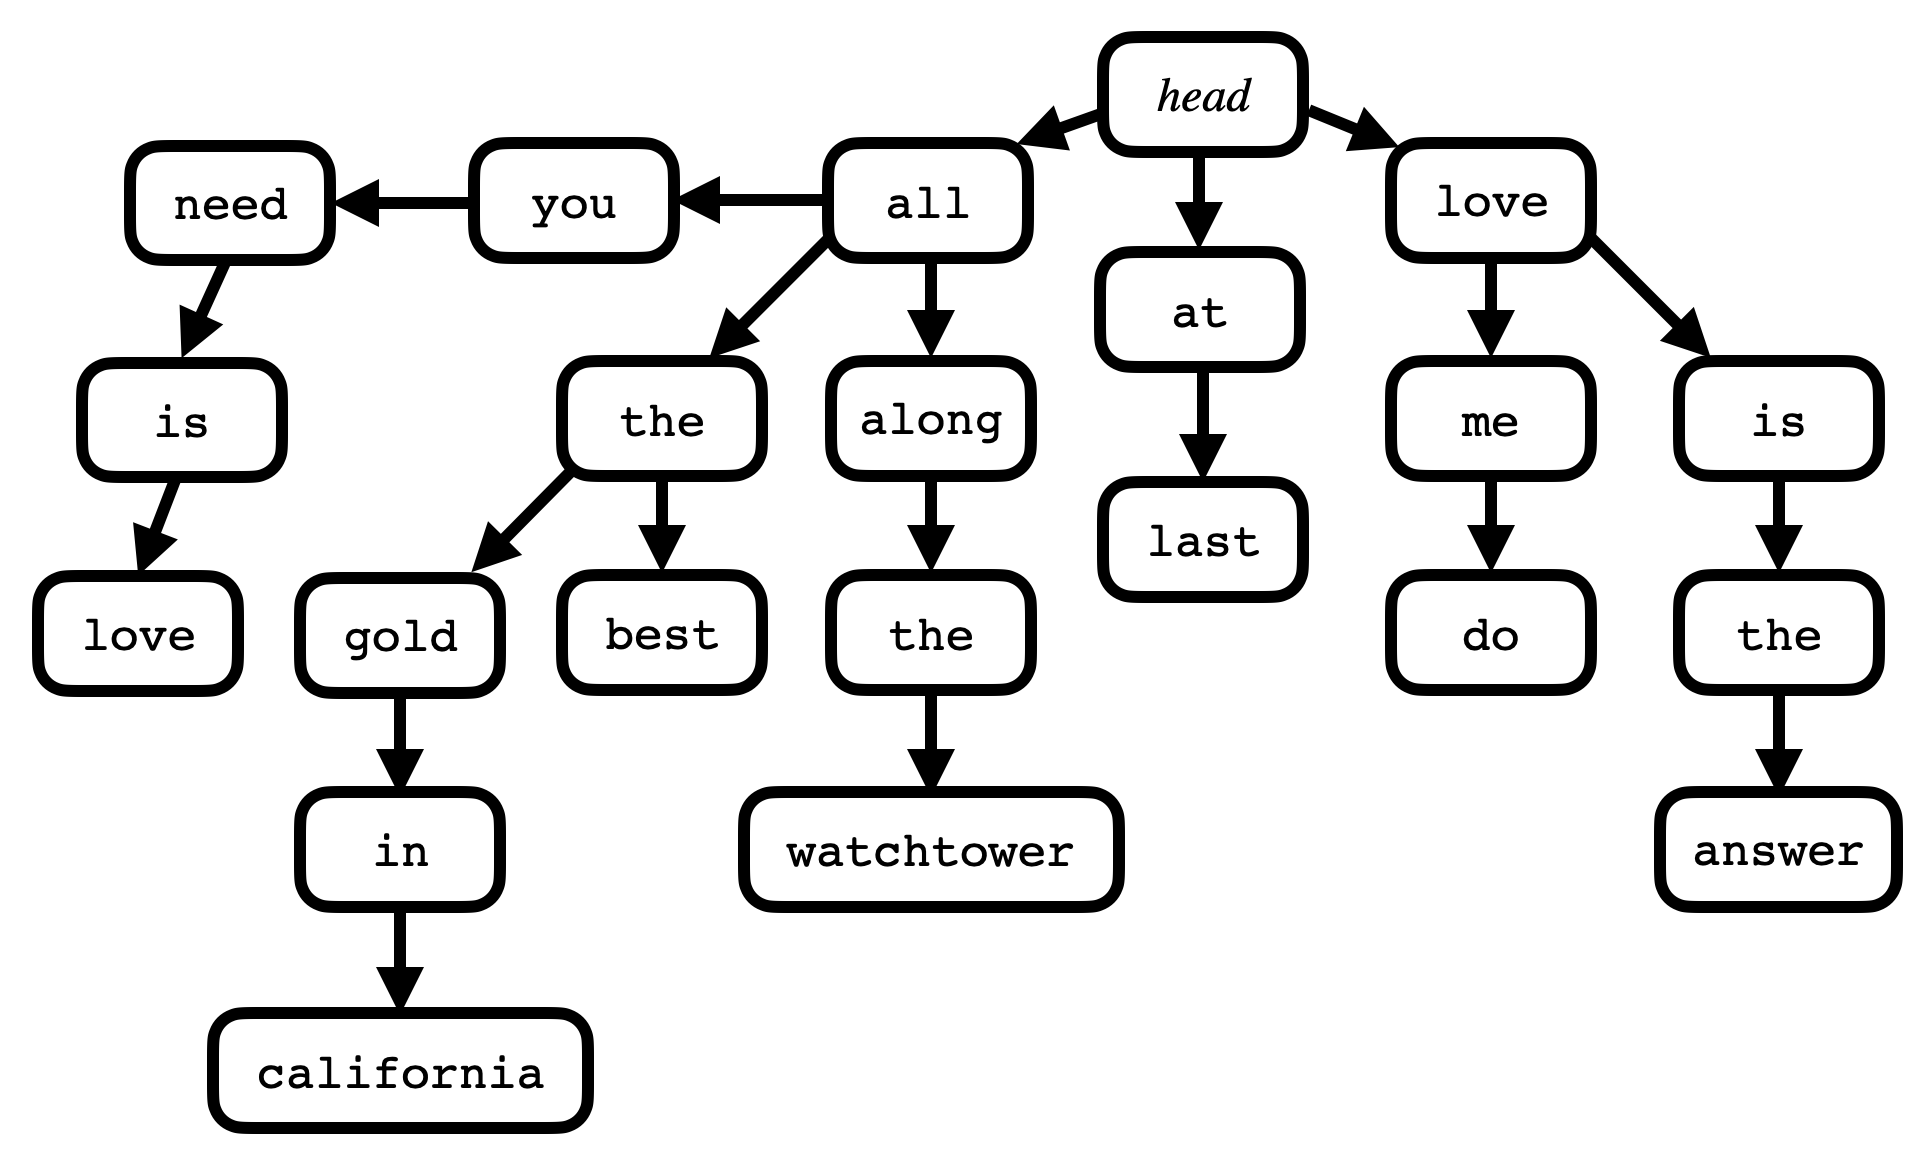
\includegraphics[width=0.8\textwidth]{content/chapter11/images/1.png}\\
Figure 11.1 – A trie of strings
\end{center}

We often start a search at the head of a trie, looking for sentences that begin with a specific word. In this example, when I search for all, I get three nodes: you, the, and along.
If I search for love, I get me and is.

A string trie is commonly used for creating search suggestions. Here we will implement a string trie using std::map for the trie structure.

\subsubsection{How to do it…}

In this recipe, we create a recursive trie class that stores nodes in a std::map container. It's a simple solution for a small in-memory trie. This is a rather large class, so we'll only show the important parts here.

For the full class, please see the source code at \url{https://github.com/ PacktPublishing/CPP-20-STL-Cookbook/blob/main/chap11/trie.cpp}.

\begin{itemize}
\item 
We have one convenience alias:

\begin{lstlisting}[style=styleCXX]
using ilcstr = initializer_list<const char *>;
\end{lstlisting}

We use ilcstr in for searching the trie.

\item 
We'll put this class in a private namespace to avoid collisions:

\begin{lstlisting}[style=styleCXX]
namespace bw {
	using std::map;
	using std::deque;
	using std::initializer_list;
\end{lstlisting}

We have a few using statements in this namespace for convenience.

\item 
The class itself is called trie. It has three data members:

\begin{lstlisting}[style=styleCXX]
class trie {
	using get_t = deque<deque<string>>;
	using nodes_t = map<string, trie>;
	using result_t = std::optional<const trie*>;
	
	nodes_t nodes{};
	mutable get_t result_dq{};
	mutable deque<string> prefix_dq{};
\end{lstlisting}

The trie class has a few local type aliases:

\begin{itemize}
\item 
get\_t is a deque of deque of string, used for string results.

\item 
nodes\_t is a map of trie classes with string keys.

\item 
result\_t is an optional of a pointer to a trie, for returning search results. An empty trie is a valid result, so we use an optional value.
\end{itemize}

The nodes object is used for holding a recursive map of nodes, where each node on a trie is another trie.

\item 
The public interface often calls utility functions in the private interface. For example, the insert() method takes an initializer\_list object and calls the private function \_insert():

\begin{lstlisting}[style=styleCXX]
void insert(const ilcstr& il) {
	_insert(il.begin(), il.end());
}
\end{lstlisting}

The private \_insert() function does the work of inserting elements:

\begin{lstlisting}[style=styleCXX]
template <typename It>
void _insert(It it, It end_it) {
	if(it == end_it) return;
	nodes[*it]._insert(++it, end_it);
}
\end{lstlisting}

This facilitates the recursive function calls necessary to navigate the trie. Note that referencing a key that does not appear in a map creates an empty element with that key. So, the line that calls \_insert() on a nodes element creates an empty trie object if the element doesn't already exist.

\item 
The get() method returns a get\_t object, which is an alias for a deque of deque of string. This allows us to return multiple sets of results:

\begin{lstlisting}[style=styleCXX]
get_t& get() const {
	result_dq.clear();
	deque<string> dq{};
	_get(dq, result_dq);
	return result_dq;
}
\end{lstlisting}

The get() method calls the private \_get() function, which recursively traverses the trie:

\begin{lstlisting}[style=styleCXX]
void _get(deque<string>& dq, get_t& r_dq) const {
	if(empty()) {
		r_dq.emplace_back(dq);
		dq.clear();
	}
	for(const auto& p : nodes) {
		dq.emplace_back(p.first);
		p.second._get(dq, r_dq);
	}
}
\end{lstlisting}

\item 
The find\_prefix() function returns a deque with all matches to a partial string.

\begin{lstlisting}[style=styleCXX]
deque<string>& find_prefix(const char * s) const {
	_find_prefix(s, prefix_dq);
	return prefix_dq;
}
\end{lstlisting}

The public interface calls the private function \_find\_prefix():

\begin{lstlisting}[style=styleCXX]
void _find_prefix(const string& s, auto& pre_dq) const {
	if(empty()) return;
	for(const auto& [k, v] : nodes) {
		if(k.starts_with(s)) {
			pre_dq.emplace_back(k);
			v._find_prefix(k, pre_dq);
		}
	}
}
\end{lstlisting}

The private \_find\_prefix() function traverses the trie recursively, comparing the prefix with beginning of each key. The starts\_with() method is new with C++20. With an older STL, you could use the find() method and check the return value for 0:

\begin{lstlisting}[style=styleCXX]
if(k.find(s) == 0) {
	...
\end{lstlisting}

\item 
The search() function returns an optional<const trie*>, aliased as result\_t. It has two overloads:

\begin{lstlisting}[style=styleCXX]
result_t search(const ilcstr& il) const {
	return _search(il.begin(), il.end());
}
result_t search(const string& s) const {
	const ilcstr il{s.c_str()};
	return _search(il.begin(), il.end());
}
\end{lstlisting}

These methods pass iterators to the private member function \_search(), which does the work of the search:

\begin{lstlisting}[style=styleCXX]
template <typename It>
result_t _search(It it, It end_it) const {
	if(it == end_it) return {this};
	auto found_it = nodes.find(*it);
	if(found_it == nodes.end()) return {};
	return found_it->second._search(++it, end_it);
}
\end{lstlisting}

The \_search() function searches recursively until it finds a match, then returns a node in the result\_t object. If it finds no match, it returns the non-value optional.

\item 
We also have two overloads of a print\_trie\_prefix() function. This function prints the contents of a trie from a prefix, used as a search key. One version uses a string for the prefix, the other uses an initializer\_list of C-strings:

\begin{lstlisting}[style=styleCXX]
void print_trie_prefix(const bw::trie& t,
		const string& prefix) {
	auto& trie_strings = t.get(\);
	cout << format("results for \"{}...\":\n", prefix);
	for(auto& dq : trie_strings) {
		cout << format("{} ", prefix);
		for(const auto& s : dq) cout << format("{} ", s);
		cout << '\n';
	}
}

void print_trie_prefix(const bw::trie& t,
		const ilcstr & prefix) {
	string sprefix{};
	for(const auto& s : prefix) sprefix +=
		format("{} ", s);
	print_trie_prefix(t, sprefix);
}
\end{lstlisting}

These functions call the get() member function to retrieve the results from the trie.

\item 
Now we can test the trie class in the main() function. First, we declare a trie and insert some sentences:

\begin{lstlisting}[style=styleCXX]
int main() {
	bw::trie ts;
	ts.insert({ "all", "along", "the", "watchtower" });
	ts.insert({ "all", "you", "need", "is", "love" });
	ts.insert({ "all", "shook", "up" });
	ts.insert({ "all", "the", "best" });
	ts.insert({ "all", "the", "gold", "in",
		"california" });
	ts.insert({ "at", "last" });
	ts.insert({ "love", "the", "one", "you're",
		"with" });
	ts.insert({ "love", "me", "do" });
	ts.insert({ "love", "is", "the", "answer" });
	ts.insert({ "loving", "you" });
	ts.insert({ "long", "tall", "sally" });
	...
\end{lstlisting}

The insert() calls pass an initializer\_list with all the strings of a sentence. Each of the strings of a sentence are inserted into the hierarchy of the trie.

\item 
Now we can search the trie. Here's a simple search for the single string "love".

\begin{lstlisting}[style=styleCXX]
const auto prefix = {"love"};
if (auto st = ts.search(prefix); st.have_result) {
	print_trie_prefix(*st.t, prefix);
}
cout << '\n';
\end{lstlisting}

This calls ts.search() with an initializer\_list of one C-string, called prefix. The result, along with the prefix, is then passed to the print\_trie\_prefix() function.

The output is:

\begin{tcblisting}{commandshell={}}
results for "love...":
love is the answer
love me do
love the one you're with
\end{tcblisting}

\item
Here's a search for a two-string prefix:

\begin{lstlisting}[style=styleCXX]
const auto prefix = {"all", "the"};
if (auto st = ts.search(prefix); st.have_result) {
	print_trie_prefix(*st.t, prefix);
}
cout << '\n';
\end{lstlisting}

Output:

\begin{tcblisting}{commandshell={}}
results for "all the ...":
all the best
all the gold in california
\end{tcblisting}

\item
And here's a search for a partial prefix, using the find\_prefix() function:

\begin{lstlisting}[style=styleCXX]
const char * prefix{ "lo" };
auto prefix_dq = ts.find_prefix(prefix);
for(const auto& s : prefix_dq) {
	cout << format("match: {} -> {}\n", prefix, s);
	if (auto st = ts.search(s); st.have_result) {
		print_trie_prefix(*st.t, s);
	}
}
cout << '\n';
\end{lstlisting}

Output:

\begin{tcblisting}{commandshell={}}
match: lo -> long
results for "long...":
long tall sally
match: lo -> love
results for "love...":
love is the answer
love me do
love the one you're with
match: lo -> loving
results for "loving...":
loving you
\end{tcblisting}

The find\_prefix() search returned several results, each of which we passed to a search of its own, resulting in several results for each result.

\end{itemize}

\subsubsection{How it works…}

The data for the trie class is stored in recursive map containers. Each node in the map contains another trie object, which in turn has its own map node.

\begin{lstlisting}[style=styleCXX]
using nodes_t = map<string, trie>
\end{lstlisting}

The \_insert() function takes begin and end iterators, and uses them to recursively call \_insert() on new nodes:

\begin{lstlisting}[style=styleCXX]
template <typename It>
void _insert(It it, It end_it) {
	if(it == end_it) return;
	nodes[*it]._insert(++it, end_it);
}
\end{lstlisting}

Likewise, the \_search() function recursively calls \_search() on the nodes it finds:

\begin{lstlisting}[style=styleCXX]
template <typename It>
result_t _search(It it, It end_it) const {
	if(it == end_it) return {this};
	auto found_it = nodes.find(*it);
	if(found_it == nodes.end()) return {};
	return found_it->second._search(++it, end_it);
}
\end{lstlisting}

This recursive approach using std::map allows us to implement a trie class concisely and efficiently.






























